\section{Experimental Evaluation} % 70/300 points, 23%

We fine-tune and evaluate the \BertSumAbs summarization model from the reproduced paper by \citeauthor{LiuL2019} on a A100 GPU using the Flux framework on Julia~\cite{InnesSFGRJKPS2018,BezansonEKS2017,LiuL2019}.
A scaled-down variant of their \TransformerAbs model, that we call \TransformerAbsTiny, is trained from scratch on a GeForce MX150 GPU for testing our evaluation workflow.
We train both models using the CNN/Daily Mail datasets, but use the preprocessed variant by \citeauthor{LiuL2019} instead of the original data by \citeauthor{HermannKGEKSB2015}~\cite{LiuL2019,HermannKGEKSB2015}.
Our implementation resembles the same encoder-decoder architecture as used by \citeauthor{LiuL2019} and uses the same \BertBase model as the pretrained encoder~\cite{LiuL2019,DevlinCLT2019}.
Though, we do not tune any hyperparameters of either the model or the optimizers.
We also reimplement the beam search algorithm from scratch.
Due to instabilities in fine-tuning and hardware constraints we were unable to train the model for the full 200\,000 steps proposed by \citeauthor{LiuL2019}.
We assume that the complex hyperparameter settings and large model size used in their paper are prone to fine-tuning issues like we experienced, a problem that has recently gained more attention~\cite{DodgeISFHS2020
,ZhangWKWA2020,AghajanyanSGGZG2020}.


Describe implementation structure/approach. (Julia/Flux, , tokenization (\Bert), model structure (encoder-decoder, beam search), hyperparameter tuning, optimizer)

\subsection{Dataset}

We train and evaluate the summarization model on the CNN / Daily Mail dataset~\cite{HermannKGEKSB2015}, but use preprocessed data released by \citeauthor{LiuL2019} along with the replicated paper.
Our implementation is designed to automatically download both the pretrained \BertBase model and the preprocessed CNN/Daily Mail datasets from the Web, no manual downloads are needed.
From the preprocessed data we extract the source article and the target summary as raw text, join sentences to normalize separators, and tokenize with \Bert's word piece tokenizer~\cite{DevlinCLT2019}.

Describe raw data format.

Describe data preprocessing. (Pre-processed dataset from \citeauthor{LiuL2019}: Sentence splitting  with Stanford CoreNLP, entities are not anonymized.)

\subsection{Abstractive Summarizaion Model}

Transformer with 6 layers, 768 hidden units, hidden size of 2048.
Train for 200\,000 steps, snapshots every 2500 steps, gradient accumulation at every step.
Choose the single best snapshot for evaluation.

Describe simple tests/examples for checking implementation correctness. (Untrained model produces nonsense summaries.)

Describe implementation memory usage, complexity, and run time performance.
The full \BertSumAbs model contains 182M trainable parameters: 27M for embeddings, 85M for the encoder's transformer layers, 47M for the decoder's transformer layers, and 23M for the generator layer.

\subsection{Fine-tuning the pretrained model}

Describe training schedule.
Two Adam optimizers with~\(\beta_1 = 0.9\) and~\(\beta_2 = 0.999\).
Learning rates:
\begin{align}
    \eta_E &= 2e^{-3} \cdot \min( \text{step}^{-0.5},\ \text{step} \cdot 20\,000^{-1.5} ) \\
    \eta_D &= 0.1 \cdot \min( \text{step}^{-0.5},\ \text{step} \cdot 10\,000^{-1.5} )
\end{align}

Presumably because of the high number of parameters to tune, training this \BertSumAbs model on a A100 GPU uses about 40GB of memory at a speed of about 9 steps per minute.
Because of the slow training speed even on a powerful GPU we had to cancel training the model after 22\,500 steps.

\subsection{Beam Search}

\subsection{Experiments}

Describe experiment reproductions.

\paragraph{Training Loss}

\begin{figure}
    \centering
    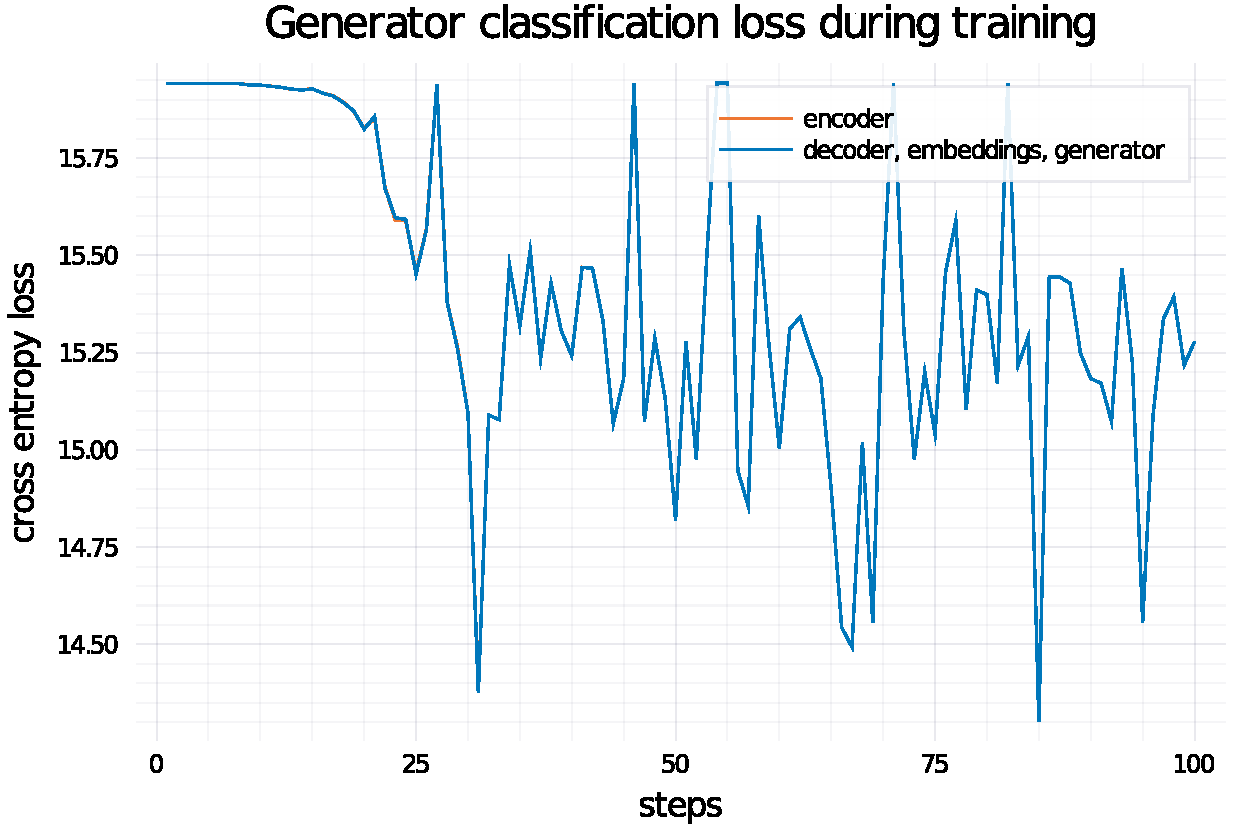
\includegraphics[width=0.7\linewidth]{training-loss-bert-abs-100.pdf}
    \caption{Cross entropy between predicted token probabilities and ground truth labels for the first 100 training steps of training the \BertSumAbs model.}
    \label{training-loss-bert-abs}
\end{figure}

\begin{figure}
    \centering
    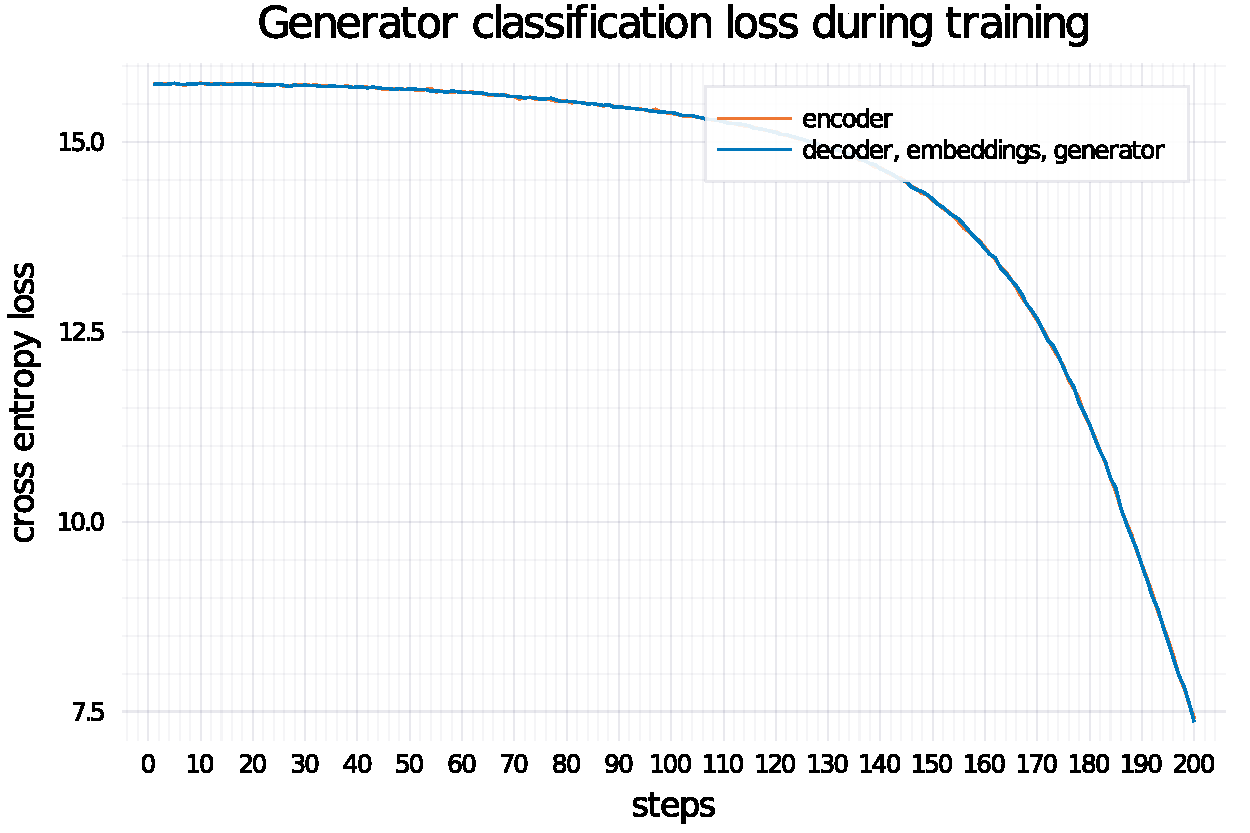
\includegraphics[width=0.7\linewidth]{training-loss-transformer-abs-tiny.pdf}
    \caption{Cross entropy between predicted token probabilities and ground truth labels for the first 200 training steps of training the \TransformerAbsTiny model.}
    \label{training-loss-transformer-abs}
\end{figure}


\paragraph{Summary Quality}

Describe \Rouge scores for some examples.

Describe/list difficulties or problems. (Pretrained data not available from a data source that allows automatic downloads.)
